% !TeX root = ../tango.tex
\section{\dispatcher{}}
\label{sec:deadline-aware-request-dispatcher}

Fig.~\ref{fig:phase-aware-deadlines} and Fig.~\ref{fig:deadline-admission-preemption} illustrate the dispatcher, which uses phase-aware deadlines as a common priority signal for request admission and preemption.
In this section, we first introduce phase-aware deadline construction (Fig.~\ref{fig:phase-aware-deadlines}), then explain how these deadlines guide waiting-queue ordering and preemption under KV-cache memory pressure (Fig.~\ref{fig:deadline-admission-preemption}).

\begin{figure}[t]
  \centering
  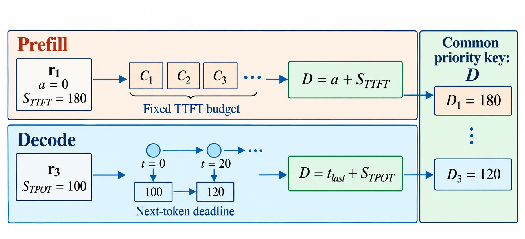
\includegraphics[width=\columnwidth]{figures/tango-methodology/phase-aware-deadlines.pdf}
  \caption{Phase-aware deadlines for request prioritization (times in ms).}
  \label{fig:phase-aware-deadlines}
  \vspace{-3mm}
\end{figure}

\subsection{Phase-Aware Request Ordering}
\label{subsec:phase-aware-request-ordering}

As analyzed in Section~\ref{subsec:motivation-underlying-reasons}, arrival order does not reflect the different latency budgets of waiting requests.
Moreover, a request's active latency objective changes during inference: before its first output token, it must produce that token within its TTFT budget; afterward, it must make timely progress in decoding.
Our key idea is to express these phase-specific objectives as an effective deadline on the same time axis.
Let $q_i$ denote the number of output tokens already returned by request $r_i$.
Using the timestamps and SLOs defined in Section~\ref{sec:multi-slo-llm-serving}, its current deadline is
\begin{equation}
\small
  D_i =
  \begin{cases}
    a_i + S_i^{\mathrm{TTFT}}, & q_i = 0, \\
    t_{i,q_i} + S_i^{\mathrm{TPOT}}, & q_i > 0.
  \end{cases}
  \label{eq:phase-aware-deadline}
\end{equation}
The first case bounds the time available before the first token, while the second gives a rolling target for the next token based on the most recent output timestamp, denoted by $t_{\mathrm{last}}$ in Fig.~\ref{fig:phase-aware-deadlines}.
Both cases map the active latency objective to the common priority key $D$, allowing the dispatcher to compare requests across inference phases.

The deadline is maintained according to output progress rather than reset whenever a request is scheduled.
During chunked prefill, all chunks share the original TTFT deadline, so both queueing and the execution of successive chunks consume the same latency budget.
For example, $r_1$ in Fig.~\ref{fig:phase-aware-deadlines} arrives at $0$~ms with a TTFT SLO of $180$~ms; its deadline remains $180$~ms across all prompt chunks.
When the first token is returned, the active objective switches to TPOT.
Each subsequent output token updates the timestamp in Eq.~\ref{eq:phase-aware-deadline} and establishes a new next-token deadline.
For $r_3$ with a TPOT SLO of $100$~ms, advancing the latest output timestamp from $0$ to $20$~ms moves its deadline from $100$ to $120$~ms.
This rolling deadline provides a local target for each inter-token interval; meeting these targets is sufficient to satisfy the average-TPOT objective in Eq.~\ref{eq:latency-metrics}.

At each iteration boundary, the dispatcher orders waiting requests by increasing $D_i$ and admits them in earliest-deadline-first (EDF) order.
Arrival time breaks deadline ties, with request identifiers providing deterministic ordering when both values are equal.
The waiting queue contains both newly arrived requests and preempted requests awaiting resumption.
A request that has not returned its first token is ranked by its TTFT deadline, while a resumed decode request is ranked by its TPOT deadline, even if recovering its context requires additional prefill work.
Admission remains subject to the engine's sequence and memory limits and the token budget supplied by the allocator.
In Fig.~\ref{fig:deadline-admission-preemption}, $r_4$ with $D_4=60$~ms is considered before $r_5$ with $D_5=200$~ms.
This ordering allows requests with later deadlines to absorb more queueing delay, giving earlier service to more urgent requests without changing their total prefill work.

\subsection{Deadline-Aware Preemption}
\label{subsec:deadline-aware-preemption}

\begin{figure}[t]
  \centering
  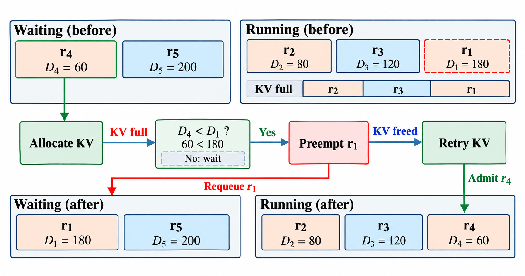
\includegraphics[width=\columnwidth]{figures/tango-methodology/deadline-admission-preemption.pdf}
  \caption{Deadline-aware admission and preemption (times in ms).}
  \label{fig:deadline-admission-preemption}
  \vspace{-3mm}
\end{figure}

During continuous batching, a new or resumed request may fail to obtain the KV-cache blocks required for admission.
The dispatcher then uses the same deadline representation to identify a running request that can yield memory.
For the current running set $\mathcal{R}_k$, it selects the candidate victim as
\begin{equation}
\small
  v = \operatorname*{arg\,max}_{i:\,r_i \in \mathcal{R}_k}
      \left(D_i, a_i\right),
  \label{eq:deadline-preemption-victim}
\end{equation}
where the tuple is compared lexicographically, so a later-arriving request is selected when deadlines are equal.
For waiting request $r_j$, preemption proceeds only if $D_j < D_v$.
Otherwise, $r_j$ remains queued, preserving the running requests whose deadlines are equally or more urgent.

When the comparison permits preemption, the engine reclaims the victim's KV-cache blocks, returns it to the waiting queue, and retries admission of $r_j$.
Preemption occurs at an iteration boundary and preserves the victim's SLOs, arrival time, output-token count, and latest output timestamp.
The victim re-enters the queue with the deadline of its current phase: its original TTFT deadline before the first token, or its existing next-token deadline afterward.
Thus, preemption does not reset the latency budget, and waiting for resumption continues to consume its remaining slack.
In the example at $t=40$~ms in Fig.~\ref{fig:deadline-admission-preemption}, KV allocation for $r_4$ fails, and $r_1$ has the latest deadline among the running requests.
Since $D_4=60$~ms is earlier than $D_1=180$~ms, the dispatcher preempts $r_1$ and admits $r_4$ after retrying allocation.
Request $r_1$ retains its $180$~ms deadline and returns to the waiting queue ahead of $r_5$, while $r_2$ and $r_3$ remain running.
